\title{TartanTrades - A Distributed Marketplace}
\author{
        Mat Gray \\
        mhgray\\
            \and
        Miko Bautista\\
        mbautist\\
}
\date{April 15, 2014}

\documentclass[12pt]{article}
\usepackage{graphicx}
\setlength{\parindent}{0cm}

\begin{document}
\maketitle

\section{Description}

TartanTrades is a system for battling the corrupt meal plan block system at CMU\@.  Currently, undergraduates are given ``blocks'' to be used to purchase meals.
These blocks expire every other week, and many go to waste since most students are unable to consume all of the blocks within the tight time limit.\\

We will solve this problem by creating a distributed marketplace that will allow for students to buy/sell their meal plan blocks.  Someone who is stuck on the meal
plan can put their blocks up for sale.  Students who are interested in purchasing a block can then send push notifications to sellers near them.  If a seller agrees
to the price that the buyer is willing to pay, the buyer and seller can meet up at one of the cafes on campus and conduct the sale.\\

There will be a rating system for buyers/sellers to ensure that people don't take advantage of others by either not paying or not having a block to sell.

\section{Implementation Structure}

We will use one master server to keep track of user authentications and other house-cleaning tasks such as maintaining a list of servers in the consistent hashing ring.\\

The following diagram shows what happens when a user wants to make a block purchase.

\begin{center}
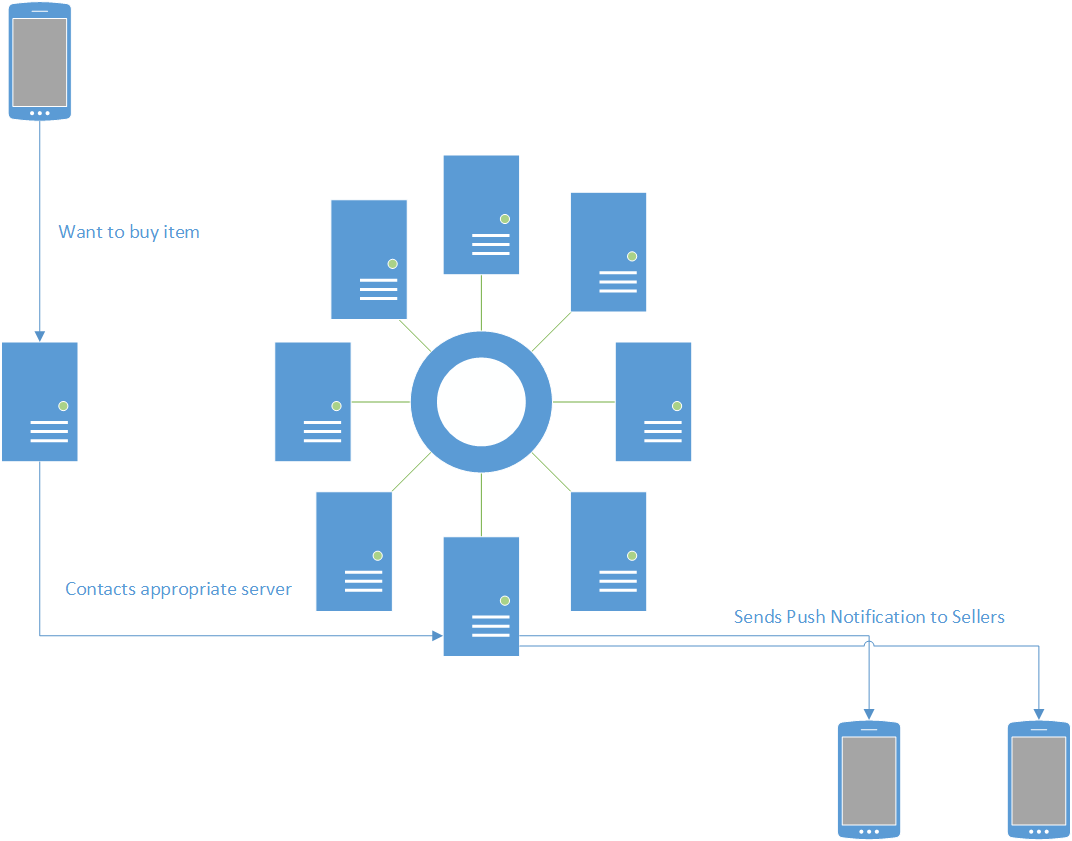
\includegraphics[scale=.6]{./diagram-1.png}\\
\end{center}

When the purchase is made, the user's phone will use Paxos to try to claim the block.  It will get a list of all the servers in the ring from the master
server then it will contact all of the servers in the ring and send the \verb|PREPARE REQUEST| message.  If no one has claimed the block yet, it will then send an \verb|ACCEPT REQUEST| in order to claim
the block.  This will guarantee that given $n$ users trying to claim a block that $1$ is given the block and $n-1$ are shown an error saying that the block has been taken.

\section{Distributed Features \& Algorithms}

TartanTrades will use Lamport timestamps in order to determine the order of events that happen.  For example, it will determine who reserved a block first.\\

On the server side, TartanTrades will use a distributed hashtable with consistant hashing to store user data and credentials.  Data for a user will be grouped onto the same server.  Moreover, the
servers will make use of replication in case a server dies.\\

TartanTrades will also make use of Paxos for handling client-side failures and also for ensuring exactly one buyer per seller (The CMU block system does not allow
for spending multiple blocks at once).  The clients will contact all of servers in the ring to try to claim the block, as discussed in the previous section.

\section{Testing}

We plan on conducting unit tests of the system's back end with the testing package built into the Go programming language. Such tests will construct an environment where several sellers and buyers are created manually. Each of them will interact with one other via API calls, getting matched up by the system accordingly.\\

We will focus on testing for output correctness for different series of calls. The system should always match up the first buyer to the first seller who accepts the deal. Tests regarding correctness involve making sure that synchronization among the servers is sustained through the use of Lamport time stamps.\\

In addition, the system should also be robust with respect to client failure. For example, if a pairing has been confirmed but the seller's machine dies, then the system should properly redirect the buyer to the next seller on the queue. If the buyer's machine dies, the system should re-add the seller at the front of the queue. Furthermore, the system should handle server failure correctly, ensuring that it recovers with accurate data once it reboots.\\

\section{Tiers}

We will divide the entire up into three main tiers, signifying varying levels of importance for the features under them to be completed. They are as follows:

\paragraph{Tier 1:}
The application should pass all tests for robustness, particularly with regard to client/server failure. It should be deployed on at least a web client and made available for CMU students. Its back-end should be fully functional - able to identify buyers/sellers on campus and pair them up accordingly. Most importantly, it should be properly build on a distributed environment with Paxos correctly implemented for node communication.

\paragraph{Tier 2:}
If time permits, we will implement mobile clients (both iOS and Android) for TartanTrades, as this will greatly increase its utility. In addition, we will also allow for different types of payment methods to be used for transactions, thus increasing its flexibility. Finally, we will implement a rating system for users to help prevent possible scams.

\paragraph{Tier 3:}
If even more time permits, we will extend TartanTrades into a generic marketplace for the campus. Not only will users be able to buy and sell blocks, but we will allow for any other item to be sold as well. This will allow for a quick and convenient way to purchase random materials on campus without having to commute too far.

\section{Schedule}

\textbf{Week of April 14th}\\
Tuesday (4/15): Proposal Due\\
Wednesday (4/16): Begin work on single server back-end\\
Friday (4/18): Extend to work for multiple servers simultaneously with Paxos\\

\textbf{Week of April 21st}\\
Monday (4/21): Continue working on making the application distributed\\
Wednesday (4/23): Preliminary demonstration\\
Thursday (4/24): Write and run test cases to ensure correctness\\
Saturday (4/26): Build front-end mobile clients\\

\textbf{Week of April 28th}\\
Monday (4/28): Extend the app to allow for different payment methods\\
Tuesday (4/29): Final demonstration\\
Wednesday (4/30): Final demonstration\\
Thursday (5/1): Final submission 

\end{document}
